\documentclass{article}
\usepackage[utf8]{inputenc}
\usepackage{fancyhdr}
\usepackage{lastpage}
\usepackage{amsfonts}
\usepackage{amsmath}
\usepackage{amsthm}
\usepackage{amssymb}
\usepackage{bm}
\usepackage{csquotes}
\usepackage{mymacros}
\usepackage{graphicx}
\usepackage{geometry}
\usepackage[shortlabels]{enumitem}
\usepackage[noabbrev, capitalise]{cleveref}

\usepackage{geometry}
 \geometry{
 a4paper,
 top=20mm,
 bottom=25mm,
 left=25mm,
 right=25mm,
 }

% define your IDs here:
\newcommand{\firststudentid}{318635646}
\newcommand{\secondstudentid}{987654321}
\newcommand{\thirdstudentid}{987654321}

\pagestyle{fancy}
\fancyhf{}
\rhead{Written Solution for Assignment 1}
\chead{\firststudentid \qquad \secondstudentid \qquad \thirdstudentid}
\lhead{Natural Language Processing}
\rfoot{Page \thepage \hspace{1pt} of \pageref{LastPage}}
\renewcommand{\footrulewidth}{1pt}
 
\setlength{\parindent}{0pt}
\setlength{\parskip}{1em}
\renewcommand{\baselinestretch}{1.25}

\renewcommand{\thesubsection}{\thesection.\alph{subsection}}
\renewcommand{\thesubsubsection}{\thesubsection.\roman{subsubsection}}

\begin{document}

\section{Understanding word2vec}
\subsection{}
\begin{proof}
  Let $\bm{x} \in \R^d$ be an input vector and let $c \in \R$ be some constant. For any $i \in [d]$ it holds that:  
  \begin{equation*}
    \begin{split}
      (\text{softmax}(\bm{x} + c))_i & = \frac{\exp(x_i + c)}{\sum_{j = 1}^{d} \exp(x_j + c)} \\
      & = \frac{e^c \exp(x_i)}{e^c \sum_{j = 1}^{d} \exp(x_j)} \\
      & = \frac{\exp(x_i)}{\sum_{j = 1}^{d} \exp(x_j)} \\
      & = (\text{softmax}(\bm{x}))_i
    \end{split}
  \end{equation*}
\end{proof}

\subsection{}
\begin{proof}
  Note that the true empirical distribution $\bm{y}$ is a one-hot vector with a 1 for the true outside word o, and 0 everywhere else, thus:
  \begin{equation*}
    -\sum\limits_{w \in \text{W}} y_w \log(\hat{y}_w) = -\sum\limits_{w \in \text{W}} \I{o}(w) \log(\hat{y}_w) = \log(\hat{y}_o)
  \end{equation*}
\end{proof}

\subsection{}
\begin{proof}
  We apply the derivative chain rule and divide into two cases depending on $w$: 
  \begin{equation}\label{eq:gradient}
    \begin{split}
      \frac{\partial \bm{J}_{\text{na\"ive-softmax}}}{\partial \bm{u}_w}(c,o,\bm{V},\bm{U}) & = -\frac{\partial \log{}}{\partial P[O=o | C-c]}(P[O=o | C=c]) \cdot \frac{\partial P[O | C=c]}{\partial \bm{u}_w}(O=o) \\
    \end{split}
  \end{equation}
  
  Note that:
  \begin{equation*}
    \frac{\partial \log}{\partial P[O=o | C-c]}(P[O=o | C-c]) = \frac{1}{P[O=o | C=c]} = \frac{\sum\limits_{w' \in \text{W}} \exp(\bm{u}_{w'}^T \bm{v}_c)}{\exp(\bm{u}_{o}^T \bm{v}_c)} 
  \end{equation*}

  \begin{description}
    \item[Case $o \neq w$:]
      \begin{equation*}
        \begin{split}
          \frac{\partial P[O | C=c]}{\partial \bm{u}_w}(O=o) 
          & =  \exp(\bm{u}_{o}^T \bm{v}_c) \left(-\left(\sum\limits_{w' \in \text{W}} \exp(\bm{u}_{w'}^T \bm{v}_c)\right)^{-2}\right) \frac{\partial}{\partial \bm{u}_w} \exp(\bm{u}_{w}^T \bm{v}_c) \\
          & = -\frac{\exp((\bm{u}_{o} + \bm{u}_{w}) ^T \bm{v}_c)} {\left(\sum\limits_{w' \in \text{W}} \exp(\bm{u}_{w'}^T \bm{v}_c)\right)^2} \cdot \bm{v}_c
        \end{split}
      \end{equation*}

      Plugging this expression into (\ref{eq:gradient}):
      \begin{equation*}
        \begin{split}
          \frac{\partial \bm{J}_{\text{na\"ive-softmax}}}{\partial \bm{u}_w}(c,o,\bm{V},\bm{U}) 
          & = \frac{\exp(\bm{u}_{w}^T \bm{v}_c)} {\sum\limits_{w' \in \text{W}} \exp(\bm{u}_{w'}^T \bm{v}_c)} \cdot \bm{v}_c \\
          & = \hat{\bm{y}}_w \cdot \bm{v}_c
        \end{split}
      \end{equation*}

      \item[Case $o = w$:]
      \begin{equation*}
        \begin{split}
          \frac{\partial P[O | C=c]}{\partial \bm{u}_o}(O=o) 
          & =  \frac{\exp(\bm{u}_{o}^T \bm{v}_c) \bm{v}_c \cdot \left(\sum\limits_{w' \in \text{W}} \exp(\bm{u}_{w'}^T \bm{v}_c)\right) \quad - \quad \exp(\bm{u}_{o}^T \bm{v}_c) \bm{v}_c \cdot \exp(\bm{u}_{o}^T \bm{v}_c)}{\left(\sum\limits_{w' \in \text{W}} \exp(\bm{u}_{w'}^T \bm{v}_c)\right)^2} \\
          & = \frac{\exp(\bm{u}_{o}^T \bm{v}_c)\left(\sum\limits_{w' \in \text{W}} \exp(\bm{u}_{w'}^T \bm{v}_c) - \exp(\bm{u}_{o}^T \bm{v}_c) \right) \bm{v}_c}{\left(\sum\limits_{w' \in \text{W}} \exp(\bm{u}_{w'}^T \bm{v}_c)\right)^2} \\
        \end{split}
      \end{equation*}

      Plugging this expression into (\ref{eq:gradient}):
      \begin{equation*}
        \begin{split}
          \frac{\partial \bm{J}_{\text{na\"ive-softmax}}}{\partial \bm{u}_o}(c,o,\bm{V},\bm{U})
          & = - \frac{\sum\limits_{w' \in \text{W}} \exp(\bm{u}_{w'}^T \bm{v}_c)}{\exp(\bm{u}_{o}^T \bm{v}_c)} \cdot \frac{\exp(\bm{u}_{o}^T \bm{v}_c)\left(\sum\limits_{w' \in \text{W}} \exp(\bm{u}_{w'}^T \bm{v}_c) - \exp(\bm{u}_{o}^T \bm{v}_c) \right) \bm{v}_c}{\left(\sum\limits_{w' \in \text{W}} \exp(\bm{u}_{w'}^T \bm{v}_c)\right)^2} \\
          & = (\hat{\bm{y}}_o - 1)\bm{v}_c \\
        \end{split}
      \end{equation*}

  \end{description}

  Thus the differential of $\bm{J}_{\text{na\"ive-softmax}}$ w.r.t $\bm{U}$ is given by:
  \begin{equation*}
    \frac{\partial \bm{J}_{\text{na\"ive-softmax}}}{\partial \bm{U}}(c,o,\bm{V},\bm{U}) = \bm{v}_c(\hat{\bm{y}} - \bm{y})^T
  \end{equation*}

\end{proof}

\subsection{}
\begin{enumerate}
  [label=(\roman*)]
  \item ${\frac{\partial \bm J_{\textrm{skip-gram}}(c, w_{t-m},\ldots w_{t+m}, \bm V, \bm U)} {\partial \bm U}} = \sum_{\substack{-m \le j \le m \\ j \ne 0}} \frac{\partial \bm{J} (\bm{v_c},w_{t+j},\bm{U})}{\partial \bm{U}}  $
  \item ${\frac{\partial \bm J_{\textrm{skip-gram}}(c, w_{t-m},\ldots w_{t+m}, \bm V, \bm U)} {\partial \bm v_c}} = \sum_{\substack{-m \le j \le m \\ j \ne 0}} \frac{\partial \bm{J} (\bm{v_c},w_{t+j},\bm{U})}{\partial \bm{v_c}}  $
  \item Assuming $\bm J_{\textrm{skip-gram}}(c, w_{t-m},\ldots w_{t+m}, \bm V, \bm U)$ is not a function of $\bm v_c$ when $w \ne c$: \\
   ${\frac{\partial \bm J_{\textrm{skip-gram}}(c, w_{t-m},\ldots w_{t+m}, \bm V, \bm U)} {\partial \bm v_w}} = \bm 0$ 
\end{enumerate}


\subsection{}
Answer taken from \cite{Goldberg2014word2vecED}: \\
One motivation for making this assumption is the following:
consider the case where both the word dog and the context dog share the same vector $\bm v$. 
Words hardly appear in the contexts of themselves, and so the model should assign a low probability to
$\Pr[dog | dog]$, which entails assigning a low value to $\bm v^T \bm v$ which is impossible.

\subsection{}
The word2vec method is based around the distributional hypothesis: 
linguistic items with similar distributions have similar meanings.
Following the derivation in \cite{Levy2014Factorization}, 
we see that the word2vec algorithm implicitly factorizes a shifted Pointwise Mutual Information matrix of the respective word and context pairs.
Applied to NLP, the PMI of two words measures how much more they co-occur, than we would have a priori expected them to appear by chance.

\section{Implementing word2vec}
\setcounter{subsection}{4}
\subsection{}
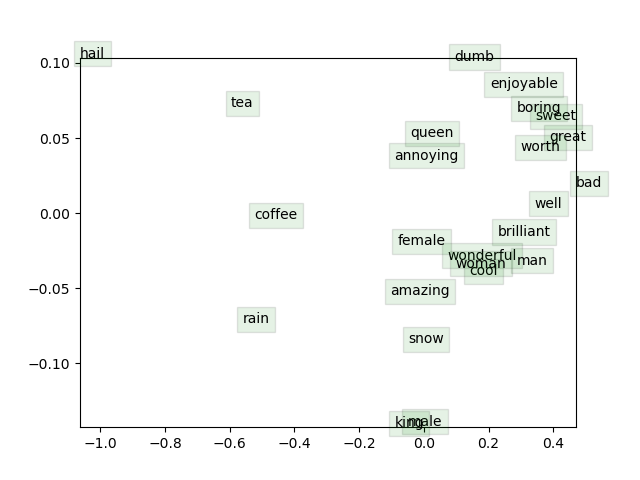
\includegraphics{word_vectors.png}

We can see some reasonable clusters in the plot, for example the words "man", "woman" and "female" have close representation.
In contrary, there are some words that were expected to be closer, such are "king", "queen" and "hail".
\section{Optimizing word2vec}
\subsection{}
\begin{proof}
    Using the first hint, we can rewrite our objection as follows:
    \begin{equation*}
            \mathcal{L}(\theta) = \prod_{c,o} p_{\theta}(o|c)^{\#(c,o)}
    \end{equation*}
    This is true because the term $p_\theta(o|c)$ by definition will appear $\#(c,o)$ times.
    Notice that for a center word $c$, the distribution of $p_theta(o|c)$ is independent from $p_\theta(o|\hat{c})$ where $c\neq\hat{c}$.
    So, we can split $\cal{L}(\theta)$ into $\cal{L}$$_c(\theta)$ such that:
    \begin{equation*}
            \mathcal{L}_c(\theta) = \prod_{o} p_{\theta}(o|c)^{\#(c,o)}
    \end{equation*}
    Taking a logarithm we get:
    \begin{equation*}
            J_c(\theta) = \sum_{o} \#(c,o)\log{p_{\theta}(o|c)}
    \end{equation*}

    Since for each $c$, $p_theta(o|c)$ is a probability distribution, we know that:
    \begin{equation*}
            \sum_{o}p_{\theta}(o|c)=1
    \end{equation*}
    So we want to solve: $J_c(\theta) = \sum_{o} \#(c,o)\log{p_{\theta}(o|c)}$ s.t $\sum_{o}p_{\theta}(o|c)=1$  and  $p_{\theta}(o|c)\ge0$

    We will solve it using Lagrange multipliers:
    \begin{equation*}
        \begin{split}
            L_c(\theta,\lambda)=\sum_{o}\#(c,o)\log{p_{\theta}(o|c)}-\lambda(\sum_{o}p_{\theta}(o|c)-1)
        \end{split}
    \end{equation*}
    \begin{equation*}
        \begin{split}
            \frac{\partial L_c}{\partial p_{\theta}(o|c)}=\frac{\#(c,o)}{p_{\theta}(o|c)}-\lambda
        \end{split}
    \end{equation*}

    So: 
    \begin{equation*}
        \frac{\partial L_c}{\partial p_{\theta}(o|c)}=0\rightarrow p_{\theta}(o|c)=\frac{\#(c,o)}{\lambda}
    \end{equation*}

    Now we can find $\lambda$ using the constrains:
    
    \begin{equation*}
        \sum_{o} p_\theta(o|c)= \sum_{o}\frac{\#(c,o)}{\lambda}=1
    \end{equation*}
    Which means that:
    \begin{equation*}
        \lambda = \sum_{o}\#(c,o)
    \end{equation*}
    So finally:
    \begin{equation*}
        p_\theta(o|c) = \frac{\#(c,o)}{\sum_{o'}\#(c,o')}
    \end{equation*}
    as desired.
\end{proof}

\subsection{}
We will now make the assumption that each word in
our vocabulary, denoted as $V = \{a, b, c, d\}$, 
is represented by a real number. Consider the corpus $T = \{”aa”, ”bb”, ”cc”, ”dd”\}$.
We will prove that achieving the optimum is impossible.
Given the result of the previous section, we will prove that we cannot achieve $ p_\theta(o|c) = \frac{\#(c,o)}{\sum_{o'}\#(c,o')}$.
\begin{proof}
    Denote the optimal probability by $ p_{\theta^*}(o|c)$.
    Notice that in our corpus $p_{\theta^*}(o|c)=1$ iff $o=c$ and $0$ otherwise.
    Assume toward contradiction that we have found a word representation that results in the optimal solution.
    By the pigeonhole principle, there must exsits two different words with the same sign, denote them by $u_c$ and $u_{c'}$.
    Assume without loss of generality that $|u_c|\le|u_{c'}|$.
    Since they have the same sign we know that $\exp{(u_cu_c)}\le\exp{(u_cu_{c'})}$.\\\\Now we get that:
    \begin{equation}\label{eq:ineq}
        p_\theta(c|c)= \frac{\exp{(u_cu_c)}}{\sum_{w\in V}\exp{(u_wu_c)}} \le \frac{\exp{(u_cu_{c'})}}{\sum_{w\in V}\exp{(u_wu_c)}} \le p_{\theta}(c|c')
    \end{equation}
    But we know that $p_\theta(c|c)=1$ and $ p_{\theta}(c|c')=0$, wich contradicts \ref{eq:ineq}.
\end{proof}

\section{Paraphrase Detection (theoretical)}
\subsection{}
\begin{align*}
    &2^{-\frac{1}{M}\sum log_2 p(s_i | s_1,...,s_{i-1})}= \\
&= (2^{\sum log_2 p(s_i | s_1,...,s_{i-1})})^{-\frac{1}{M}}= \\
&= (\prod 2^{log_2 p(s_i | s_1,...,s_{i-1})})^{-\frac{1}{M}}= \\
&= (\prod p(s_i | s_1,...,s_{i-1}))^{-\frac{1}{M}}= \\
&= (\prod e^{ln p(s_i | s_1,...,s_{i-1})})^{-\frac{1}{M}}= \\
&= e^{-\frac{1}{M}\sum ln p(s_i | s_1,...,s_{i-1})}
\end{align*}
\subsection{}
The simplest solution is to remove the relus, i.e $\sigma(x_1^T x_2)$.
If we have to keep the relu functions at the last layer, then we can map the sigmoid into $[0,1]$ by adding this computation
$$2*(\sigma (relu(x_1)^T relu(x_2)) - 0.5)$$
\newpage
\bibliography{main}
\bibliographystyle{abbrv}

\end{document}